\documentclass[border=4pt]{standalone}

\usepackage{amsmath}
\usepackage{tikz}
\usepackage{mathdots}
\usepackage{yhmath}
\usepackage{cancel}
\usepackage{color}
\usepackage{siunitx}
\usepackage{array}
\usepackage{multirow}
\usepackage{amssymb}
\usepackage{gensymb}
\usepackage{tabularx}
\usepackage{booktabs}
\usetikzlibrary{fadings}
\usetikzlibrary{patterns}
\usetikzlibrary{shadows.blur}
\usetikzlibrary{shapes}
 

\begin{document}



\tikzset{every picture/.style={line width=0.75pt}} %set default line width to 0.75pt        

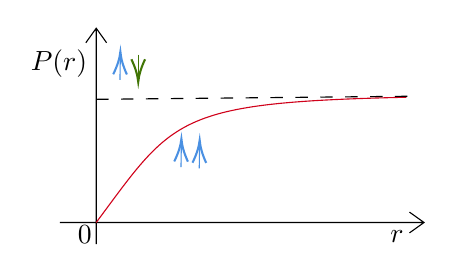
\begin{tikzpicture}[x=0.75pt,y=0.75pt,yscale=-1,xscale=1]
%uncomment if require: \path (0,300); %set diagram left start at 0, and has height of 300

%Shape: Axis 2D [id:dp9846934458718419] 
\draw  (52,140.1) -- (227.5,140.1)(69.55,46.5) -- (69.55,150.5) (220.5,135.1) -- (227.5,140.1) -- (220.5,145.1) (64.55,53.5) -- (69.55,46.5) -- (74.55,53.5)  ;
%Curve Lines [id:da1805837339052052] 
\draw [color={rgb, 255:red, 208; green, 2; blue, 27 }  ,draw opacity=1 ]   (69.55,140.1) .. controls (107,89.75) and (107.5,82.25) .. (219,79.75) ;
%Straight Lines [id:da1940926030483967] 
\draw  [dash pattern={on 4.5pt off 4.5pt}]  (69.5,80.75) -- (221.5,79.25) ;
%Straight Lines [id:da8678559062807047] 
\draw [color={rgb, 255:red, 74; green, 144; blue, 226 }  ,draw opacity=1 ]   (81,71.4) -- (81.17,59.8) ;
\draw [shift={(81.2,57.8)}, rotate = 450.84] [color={rgb, 255:red, 74; green, 144; blue, 226 }  ,draw opacity=1 ][line width=0.75]    (10.93,-3.29) .. controls (6.95,-1.4) and (3.31,-0.3) .. (0,0) .. controls (3.31,0.3) and (6.95,1.4) .. (10.93,3.29)   ;
%Straight Lines [id:da7684783270546323] 
\draw [color={rgb, 255:red, 74; green, 144; blue, 226 }  ,draw opacity=1 ][fill={rgb, 255:red, 74; green, 144; blue, 226 }  ,fill opacity=1 ]   (110.4,113.4) -- (110.57,101.8) ;
\draw [shift={(110.6,99.8)}, rotate = 450.84] [color={rgb, 255:red, 74; green, 144; blue, 226 }  ,draw opacity=1 ][line width=0.75]    (10.93,-3.29) .. controls (6.95,-1.4) and (3.31,-0.3) .. (0,0) .. controls (3.31,0.3) and (6.95,1.4) .. (10.93,3.29)   ;
%Straight Lines [id:da9785433881452457] 
\draw [color={rgb, 255:red, 74; green, 144; blue, 226 }  ,draw opacity=1 ]   (119.2,114) -- (119.37,102.4) ;
\draw [shift={(119.4,100.4)}, rotate = 450.84] [color={rgb, 255:red, 74; green, 144; blue, 226 }  ,draw opacity=1 ][line width=0.75]    (10.93,-3.29) .. controls (6.95,-1.4) and (3.31,-0.3) .. (0,0) .. controls (3.31,0.3) and (6.95,1.4) .. (10.93,3.29)   ;
%Straight Lines [id:da20614739444588204] 
\draw [color={rgb, 255:red, 65; green, 117; blue, 5 }  ,draw opacity=1 ]   (89.8,59.2) -- (89.8,70.4) ;
\draw [shift={(89.8,72.4)}, rotate = 270] [color={rgb, 255:red, 65; green, 117; blue, 5 }  ,draw opacity=1 ][line width=0.75]    (10.93,-3.29) .. controls (6.95,-1.4) and (3.31,-0.3) .. (0,0) .. controls (3.31,0.3) and (6.95,1.4) .. (10.93,3.29)   ;

% Text Node
\draw (59.5,140.4) node [anchor=north west][inner sep=0.75pt]    {$0$};
% Text Node
\draw (210,142.6) node [anchor=north west][inner sep=0.75pt]    {$r$};
% Text Node
\draw (36.8,55.6) node [anchor=north west][inner sep=0.75pt]    {$P(r)$};


\end{tikzpicture}

\end{document}
